%% @Author: KEMKA TAKENGNY Ulrich
%  @Date:   2024-08
%% @Class:  PFE IMIE-PARIS.

\documentclass[a4paper, oneside, 12pt, final]{extreport}
\usepackage{mathptmx}
\usepackage{graphicx}

\parindent 1cm
\usepackage{makeidx}
\makeindex
\usepackage[lined,boxed,commentsnumbered, english, ruled,vlined,linesnumbered, french]{algorithm2e}
\usepackage{amsthm}
\usepackage{float}
\usepackage{subcaption}
\usepackage{multirow}
\usepackage{array}




\providecommand{\keywords}[1]{\textbf{\textit{Mots clés---}} #1}
\providecommand{\keywordss}[1]{\textbf{\textit{Keywords---}} #1}


\usepackage{etoolbox}

% Pour l'interligne
\usepackage{setspace}

% Configurer l'interligne à 1.5
\onehalfspacing

\usepackage[nottoc]{tocbibind}

\textwidth 16.5cm
\textheight 24cm
\topmargin -1cm
\oddsidemargin -0.3cm

% set font encoding for PDFLaTeX or XeLaTeX
\usepackage{ifxetex}
\ifxetex
  \usepackage{fontspec}
\else
  \usepackage[T1]{fontenc}
  \usepackage[utf8]{inputenc}
  \usepackage{lmodern}
\fi

% Ajouter hyperref pour les liens cliquables
\usepackage[hidelinks]{hyperref}

\setcounter{secnumdepth}{3}


% Enable SageTeX to run SageMath code right inside this LaTeX file.
% documentation: http://mirrors.ctan.org/macros/latex/contrib/sagetex/sagetexpackage.pdf
%\usepackage{sagetex}


\newcommand{\reportTitle} {
  \textsc{Projet de Fin d'\'etudes}
}

\newcommand{\reportAuthor} {
  \textbf{Ulrich KEMKA TAKENGNY}
}

\newcommand{\reportSubject} {
  Développement et optimisation des plateformes de simulation pour les scénarios de sécurité et défense : \textit{IntelLab} 
}


\newcommand{\IMIE} {%
\\ Ecole Supérieure d'informatique IMIE-Paris
}

\newcommand{\AU} {
\centering \textbf{Année Académique 2023-2024}
}

\newcommand{\specialcell}[1]{%
  \begin{tabularx}{\textwidth}{@{}X@{}}#1\end{tabularx}%
}

%%%%%%%%%%%%%%%%%%%%%%%%%%%%%%%%%%%%%%%%%%%%%%%%%%%%%%%
% Add your own commands here
%%%%%%%%%%%%%%%%%%%%%%%%%%%%%%%%%%%%%%%%%%%%%%%%%%%%%%%
\newcommand{\MyCommand} {%
  Does nothing really%
}

\renewcommand{\chaptername}{Chapitre}
\renewcommand{\contentsname}{Table des matières}
\renewcommand{\listfigurename}{Liste des Figures}
% \renewcommand{\listtablename}{Liste des Tableaux}

% used in maketitle
\title{\reportSubject}
\author{\reportAuthor}

% Enable SageTeX to run SageMath code right inside this LaTeX file.
% documentation: http://mirrors.ctan.org/macros/latex/contrib/sagetex/sagetexpackage.pdf


\usepackage{graphics}
\usepackage{graphicx}

\usepackage[acronym,toc,section=chapter]{glossaries}
\makeglossaries

\newacronym{abc}{ABC}{A contrived acronym}
\newacronym{efg}{EFG}{Another acronym}
\newacronym{svm}{SVM}{Support Vector Machines}

\pagenumbering{roman}

\usepackage[utf8]{inputenc}

\begin{document}
\thispagestyle{empty}
\begin{titlepage}
  \begin{center}
    %%%%%%%%%%%%%%%%%%%%%%%%%%%%%%%%%%%%%%%%%%%%%%%
    % THE HEADER
    %%%%%%%%%%%%%%%%%%%%%%%%%%%%%%%%%%%%%%%%%%%%%%%

    
\includegraphics[scale=0.7]{./images/inr_logo_rouge.png}
    \hfill
    
\includegraphics[scale=0.4]{./images/logonoir.png}

    \vspace{3cm}

    %%%%%%%%%%%%%%%%%%%%%%%%%%%%%%%%%%%%%%%%%%%%%%%
    % THE PAGE CONTENT
    %%%%%%%%%%%%%%%%%%%%%%%%%%%%%%%%%%%%%%%%%%%%%%%

    \textbf{\textit{Rapport d'activité de fin d'alternance}}\\

    \vspace{5pt}
    {\textit{Réalisé par}}\\
    \vspace{10pt} {
      \fontsize{14pt}{14pt}\selectfont
      {\bfseries\Large\sc \reportAuthor}\\
    }

    \vspace{15pt}

    {
      \renewcommand*{\familydefault}{\defaultFont}
      \fontsize{27pt}{27pt}\selectfont%
      \rule{0.5\textwidth}{.4pt}\\
      \vspace{10pt}
      \reportSubject{}\\%
      \vspace{10pt}
      \rule{0.5\textwidth}{.4pt}
    }

    \vspace{30pt}
    {Diplôme préparé : \textbf{\large Manager de Solutions Digitales et Data}}\\
    \vspace{46pt}

    Sous la supervision de :  \textbf{Jonas RENAULT}, \textit{Chef de projet informatique}\\
    \vspace{50pt}

  \end{center}
  \vspace{30pt}
  \AU\\
\end{titlepage}


%%%%%%%%%%%%%%%%%%%%%%%%%%%%%%%%%%%%%%%%%%%%%%%%%%%%%%%
% Divers chapitres
%%%%%%%%%%%%%%%%%%%%%%%%%%%%%%%%%%%%%%%%%%%%%%%%%%%%%%%

\tableofcontents
\addcontentsline{toc}{chapter}{Table des matières}

\listoffigures


\cleardoublepage

\newpage
\pagenumbering{arabic}
\chapter*{Introduction}
\label{chap:general_intorduction}



\markboth{\MakeUppercase{Introduction}}{}%
\addcontentsline{toc}{chapter}{Introduction}%

%Welcome to \Ac{ITBS}. ~\\
%Again, welcome to \Ac{ITBS}. ~\\
%Your introduction goes here. ~\\

Voici une référence à l'image de la Figure \ref{fig:test} page \pageref{fig:test} et une autre vers la partie \ref{chap:2} page \pageref{chap:2}.
On peut citer un livre\, \cite{caillois1} et on précise les détails à la fin du rapport dans la partie références.
Voici une note\,\footnote{Texte de bas de page} de bas de page\footnote{J'ai bien dit bas de page}. Nous pouvons également citer l'Algorithme , la Définition \ref{def1}, le Théorème \ref{theo1} ou l'Exemple \ref{exo1}...\\

Le document est détaillé comme suit : le chapitre \ref{chap:chapterone} introduit le cadre général de ce travail. Il s'agit de présenter l'entreprise d'accueil et de détailler la problématique. Le chapitre \ref{chap:2} introduit les données ainsi que les modèles choisies.\\


Dans le cadre de notre formation et en tant qu’alternant, nous sommes partagés entre les
enseignements à l’école et les enseignements en entreprise, ceci pour faciliter notre immersion
dans le monde du travail. Pour mon alternance, j’ai intégré le centre de recherche Inria, dans le département Mission Défense et Sécurité en tant que Développeur Web
Au cours de cette expérience professionnelle, j’ai participé au développement d'une application web permettant contenant des scénarios permettant de simuler l'exploitation du renseignement d'intérêt militaire,
au déploiement d'un mail serveur simulant un scénario de sécurité économique dans un environnement d'entreprise (startup, équipe projet recherche) et
à l'optimisation des Algorithmes de Deep Learning pour la Détection et la Reconnaissance en Temps Réel de Véhicules  Militaires dans des Images et Vidéos
Ces projets dont l’objectif d’une part à faire appréhender aux académiques et aux entreprises les problèmes
concrets rencontrés par les opérationnels afin d’y proposer des solutions communes, et
d’autre part, de permettre d’expérimenter les solutions sur la base de procédures de tests
« opérationnels » constitueront la pierre angulaire notre rapport.



\chapter{Présentation de l'entreprise}
\label{chap:chapterone}
%%%%%%%%%%%%%%%%%%%%%%%%%%%%
% SECTION                  %
%%%%%%%%%%%%%%%%%%%%%%%%%%%%
\section{Présentation du centre de recherche}
\label{chap:sectionone}

\subsection{Inria : métiers et chiffres clés.}

L’Inria est l’institut national de recherche en sciences et technologies du numérique, crée en 1967, il dispose de 11 centres et plus de 20 antennes et emploie 2600 personnes. La recherche de rang mondial, l’innovation technologique et le risque entrepreneurial constituent son ADN.
Au sein de 215 équipes-projets en général communes avec des partenaires académiques, plus de 3 900 chercheurs et ingénieurs y explorent des voies nouvelles. 900 personnels d’appui à la recherche et à l’innovation contribuent à faire émerger et grandir des projets scientifiques ou entrepreneuriaux qui impactent le monde.

L’institut fait appel à de nombreux talents dans plus d’une quarantaine de métiers différents, travaille avec de nombreuses entreprises et a accompagné la création de plus de 180 start-ups.
Inria soutient la diversité des voies de l’innovation : de l’édition open source de logiciels à la création de startups technologiques (Deeptech).


\subsection{Le service de l’apprenti : Mission Défense et Sécurité}

Le renforcement des partenariats avec la sphère Sécurité/Défense de l’État est une priorité stratégique de l’Inria. C’est de ce contexte qu’est né l’institut. Créé en mars 2020 et dirigé par Frédérique Segond, la Mission Défense et Sécurité a pour objectif le soutient des politiques gouvernementales qui visent la souveraineté et l’autonomie stratégique numérique de l’Etat français, voire européen. Elle fédère tous les projets sécurité défense d’Inria bientôt de toute la France.
L’équipe en pleine croissance est actuellement composée de seize personnes ayant chacun un rôle bien définit avec le soutien des intervenants externes à la mission.

\section{Description du projet IntelLab}
\subsection{Contexte}

Les ambitions de la mission sont aujourd’hui implémentées à travers deux structures

\begin{itemize}\addtolength{\itemsep}{-0.35\baselineskip}
  \item IntelLab, un environnement de \textbf{simulation, formation, et d’expérimentation}, il vise d’une part à faire appréhender aux académiques et aux entreprises les problèmes concrets rencontrés par les opérationnels afin d’y proposer des solutions communes, et d’autre part, de permettre d’expérimenter les solutions sur la base de procédures de tests « opérationnels ».
  \item Un centre d’excellence dédié au domaine de la Sécurité / Défense afin de faciliter le développement et le transfert à court, moyen et long terme de technologies issues de la Recherche.
\end{itemize}

\noindent Entre autres, La plateforme IntelLab permet de jouer différents types de scénario :

\begin{itemize}\addtolength{\itemsep}{-0.35\baselineskip}%
  \item Des scénarios simulant l'exploitation du renseignement d'intérêt militaire ;
  \item Un scénario de Lutte Informatique d'influence (L2I) ;
  \item Des scénarios de détection de signaux faibles précurseurs d'actions d'ingérence.
\end{itemize}

\subsection{Principales activités}


Sous la supervision du responsable informatique, j'ai développé divers outils pédagogiques et technologiques visant à faciliter la prise en main des applications et à enrichir la compréhension des scénarios d'exercice de simulation. Mon travail a contribué à l'élaboration et à l'optimisation de nouvelles technologies au sein de l'équipe.

J'ai principalement participé au développement et à l'évolution de la plateforme IntelLab, un projet clé permettant de simuler des scénarios de sécurité variés.
Nous avons travaillé en mode projet avec la méthode Agile, ce qui nous a permis d'assurer une gestion efficace et un suivi optimal des projets.

\noindent Mes contributions se sont réparties sur trois projets distincts :

\begin{itemize}\addtolength{\itemsep}{-0.35\baselineskip}%
  \item \textbf{Développement de l'application web IntelLab }: J'ai pris en charge le développement des interfaces web Frontend et Backend de la plateforme, intégrant les dernières technologies pour garantir une performance et une expérience utilisateur optimales.
  \item \textbf{Mise en place d'un serveur de messagerie} : En parallèle, j'ai contribué au déploiement d'une plateforme dédiée à la simulation de scénarios de sécurité économique, centrée sur la gestion d'un serveur de messagerie. Cette plateforme est utilisée dans des exercices de simulation reproduisant des environnements d'entreprises tels que des startups ou des équipes de recherche.
  \item \textbf{Détection et reconnaissance, proche du temps réel, de véhicules militaires sur des images et vidéos} : J'ai participé à un projet visant à développer et affiner des algorithmes de Deep Learning pour la détection et la reconnaissance en temps quasi réel de véhicules militaires dans des images et vidéos.
\end{itemize}

\noindent Dans le cadre de ces projets, mes responsabilités incluent :

\begin{itemize}\addtolength{\itemsep}{-0.35\baselineskip}%
  \item \textbf{Développement web Frontend et Backend} : Conception et implémentation des fonctionnalités sur les deux volets de l'application.
  \item \textbf{Développement d'algorithmes génératifs} : Création et intégration d'algorithmes destinés à enrichir les jeux de données pour améliorer les performances des modèles.
  \item \textbf{Rédaction des tests} : Rédaction et exécution de tests pour garantir la fiabilité et la robustesse des solutions développées.
  \item \textbf{Mise en production} : Déploiement des solutions dans l'environnement de production, assurant leur bon fonctionnement et leur maintenance.
  \item \textbf{Maintenance des applications et de leurs infrastructures} : Assurer la stabilité et la disponibilité continue des applications en identifiant et résolvant les problèmes techniques rapidement.
\end{itemize}



\chapter{Présentation des projets - Analyse - Résultats obtenus}
\label{chap:2}

  

\begin{itemize}
	\item The individual \index{Entries}{entries} are indicated with a black dot, a so-called bullet.
	\item The text in the entries may be of any length.
\end{itemize}

\begin{theorem}\label{theo1}
Soit $n$ un entier naturel. Si $n$ est premier alors il n'est divisible que par 1 et par lui-même.
\end{theorem}

\begin{proof}
Here is my proof.
\end{proof}

\begin{definition}\label{def1}
Soit $A$ une courbe...
\end{definition}

Ici, il s'agit de l'utilisation de TB %\nomenclature[TB]{TB}{Très Bien} qui consiste à parler Très Bien. 
\gls{abc} et \gls{efg} sont des acronyms et des abbréviations... La méthode \gls{svm} est également couramment utilisée.

\begin{exemple}\label{exo1}
On considère le cas particulier... 
\end{exemple}

\chapter{Analyse des défis et des enseignements}
\label{chap:3}
\chapter{Projet :  Détection et reconnaissance de véhicules militaires sur des images et vidéos (DetReco)}
\label{chap:3}
\sloppy

\section{Définition}

Avant de commencer le travail effectué, nous allons rappeler les éléments sur lesquels porte le projet.
\subsection{Détection}
La détection est la capacité à distinguer un objet du fond. Le critère d'évaluation est la distance maximale à laquelle se perçoit l'objet. La détection à longue distance ne permet pas la reconnaissance de la cible, seulement d'en détecter la présence.

Pour entraîner un algorithme de détection, il faut fournir des images présentant l'objet cible à la distance maximale visée. On définit la taille des cibles pixels minimum nécessaires pour la détection. Ainsi, pour la détection, il faudra au minimum \textbf{4x8 pixels}.


\subsection{Reconnaissance}

La reconnaissance est la capacité à classifier un objet dans une catégorie. Le critère d'évaluation est la distance maximale à laquelle l'objet peut être reconnu correctement. La taille minimale nécessaire pour la reconnaissance est d'au moins \textbf{20x40 pixels}.

La reconnaissance nécessite la définition d'une classification des véhicules cibles. Plusieurs pistes ont été proposées par la DGA TT : classification des véhicules par catégories (véhicules blindés, moyens anti-char, artillerie sol-sol, etc.). La difficulté pour l'établissement d'une classification vient de l'ambiguïté des classes assignables à certaines catégories. Notamment, un véhicule d'une même catégorie peut avoir différentes fonctions, raison pour laquelle une classification par catégorie élargie est à privilégier.


\subsection{Identification}

L'identification est la capacité à identifier précisément un objet cible. L'identification par enregistrement s'appuie sur des clés d'identification spécifiques pour chaque matériel. Dans le cadre de ce projet, l'identification est laissée hors périmètre.


\section{Modèles d'entraînement}

Les algorithmes de l’état de l’art proposés dans le cadre de ce projet sont :

\begin{itemize}
    \item Pour la détection : \textbf{YoloVx} \cite{jocher2023yolo}, \textbf{Faster RCNN} \cite{ren2016faster}, \textbf{Grounding DINO} \cite{liu2023grounding}.
    \item Pour le suivi d’objets (tracking) : \textbf{DeepSort} \cite{wojke2017simple}, \textbf{ByteTrack} \cite{zhang2022bytetrack}.
\end{itemize}

Dans le cadre de ce projet, nous avons implémenté un algorithme qui s’appuie sur le modèle \textbf{YOLOv8} pour la détection et l’algorithme \textbf{DeepOCsort} \cite{maggioolino2023deep} pour le tracking de véhicules.\\

De base, nous utilisons le modèle \textbf{yolov8m.pt} (medium), qui offre un bon compromis entre taille et vitesse, mais d'autres modèles que nous utiliserons pour l'expérience, sont disponibles auprès \textit{d'ultralytics}.

\begin{table}[H]
    \centering
    \begin{tabular}{|p{2cm}|p{2cm}|p{1.7cm}|p{2.4cm}|p{2.4cm}|p{1.7cm}|p{1.7cm}|}
        \hline
        \textbf{Model}   & \textbf{Size (pixels)} & \textbf{mAP\textsuperscript{val} 50-95} & \textbf{Speed CPU ONNX (ms)} & \textbf{Speed A100 TensorRT (ms)} & \textbf{Params (M)} & \textbf{FLOPs (B)} \\ \hline
        \textit{YOLOv8n} & 640                    & 37.3                                    & 80.4                         & 0.99                              & 3.2                 & 8.7                \\ \hline
        \textit{YOLOv8s} & 640                    & 44.9                                    & 128.4                        & 1.20                              & 11.2                & 28.6               \\ \hline
        \textit{YOLOv8m} & 640                    & 50.2                                    & 234.7                        & 1.83                              & 25.9                & 78.9               \\ \hline
        \textit{YOLOv8l} & 640                    & 52.9                                    & 375.2                        & 2.39                              & 43.7                & 165.2              \\ \hline
        \textit{YOLOv8x} & 640                    & 53.9                                    & 479.1                        & 3.53                              & 68.2                & 257.8              \\ \hline
    \end{tabular}
    \caption{Comparaison des modèles YOLOv8 \cite{jocher2023yolo}}
    \label{tab:yolov8_comparaison}
\end{table}




\section{Constitution d’une base de données d’entraînement}

Cette partie du travail a pour objectif la création d'une base de données d’images permettant l’entraînement d’un algorithme de détection et reconnaissance de véhicules militaires à l'état de l'art.

Il s’agit d’identifier un algorithme cible de l’état de l’art pouvant servir de référence pour l’évaluation de la qualité du jeu de données, et d’identifier les caractéristiques du jeu de données pertinentes pour la qualité du modèle entraîné.
En effet, les modèles de deep-learning visés par la convention DetReco sont fortement sensibles aux jeux de données utilisés pour les entraîner.
Les caractéristiques qui peuvent jouer sur la qualité du modèle entraîné sont :

\begin{itemize}
    \item dimensions et résolutions des images,
    \item luminosité,
    \item dimensions et nombre des objets cibles à détecter dans l’image (gros plan, arrière plan, etc.),
    \item visibilité de l’objet cible (occulté, ou bien peu visible en raison des conditions de la mise en scène telles que brouillard, pluie, neige, fumée, obstacles, etc.),
    \item diversité et représentativité des classes.
\end{itemize}

Un algorithme qui n’aurait été entraîné que sur un sous-ensemble des données possibles serait inapte à détecter les véhicules dans des conditions qu’il ne connaît pas.
Ainsi,pour pouvoir détecter des objets dans des conditions de terrain réelles, il est nécessaire de constituer un jeu de données au plus proche possible de ces conditions



\subsection{Définition des classes}

Afin de développer un modèle capable de faire la différence entre différents types de véhicules militaires, nous allons classifier les véhicules.

La définition d’une classification pose problème en raison de l’ambiguïté des véhicules pouvant se retrouver dans plusieurs classes.
Une première classification a été proposée pour regrouper les véhicules dans des catégories larges :

Nous utiliserons 4 classes :

\begin{itemize}
    \item Armoured Fighting Vehicle \textbf{(AFV) :} véhicules blindés de combat. (Figure \ref{fig:afv})
    \item Armoured Personnel Carrier \textbf{(APC) :} véhicules blindés pour transport des troupes. (Figure \ref{fig:apc})
    \item Military Engineering Vehicle \textbf{(MEV) :} véhicules conçu pour les travaux de construction. (Figure \ref{fig:mev})
    \item Light armoured vehicle \textbf{(LAV) :} véhicules blindés légers. (Figure \ref{fig:lav})
\end{itemize}
Cette classification pourra être amendée en fonction des résultats obtenus par l’algorithme de détection et de l’expertise de la DGA TT.


\begin{figure}[H]
    \centering
    \begin{subfigure}[b]{0.45\textwidth}
        \centering
        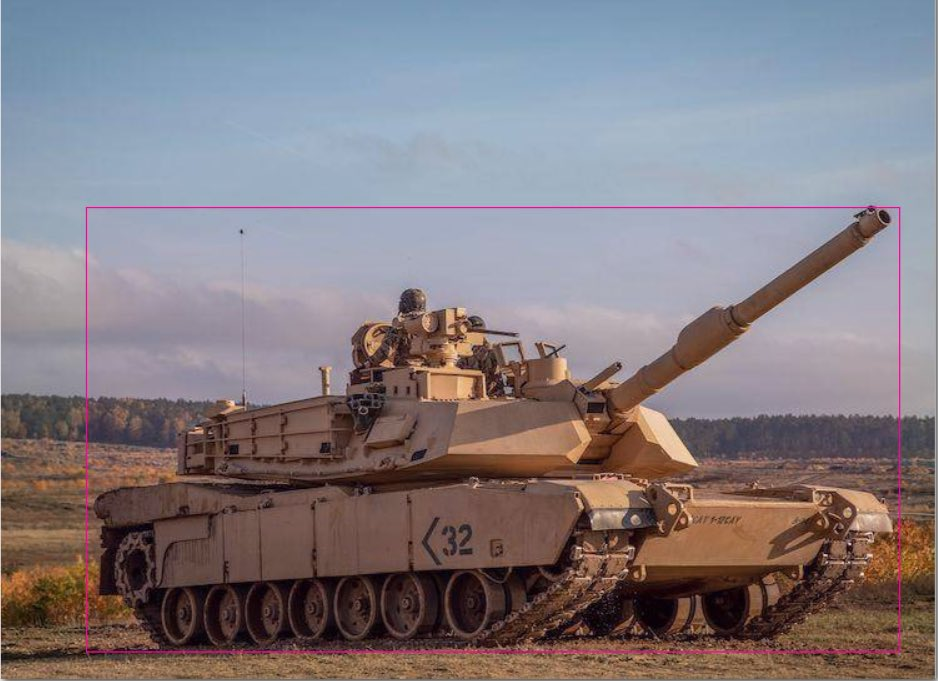
\includegraphics[width=\textwidth]{./images/afv.png}
        \caption{\textbf{AFV} - char M1 Abrams}
        \label{fig:afv}
    \end{subfigure}
    \hfill
    \begin{subfigure}[b]{0.45\textwidth}
        \centering
        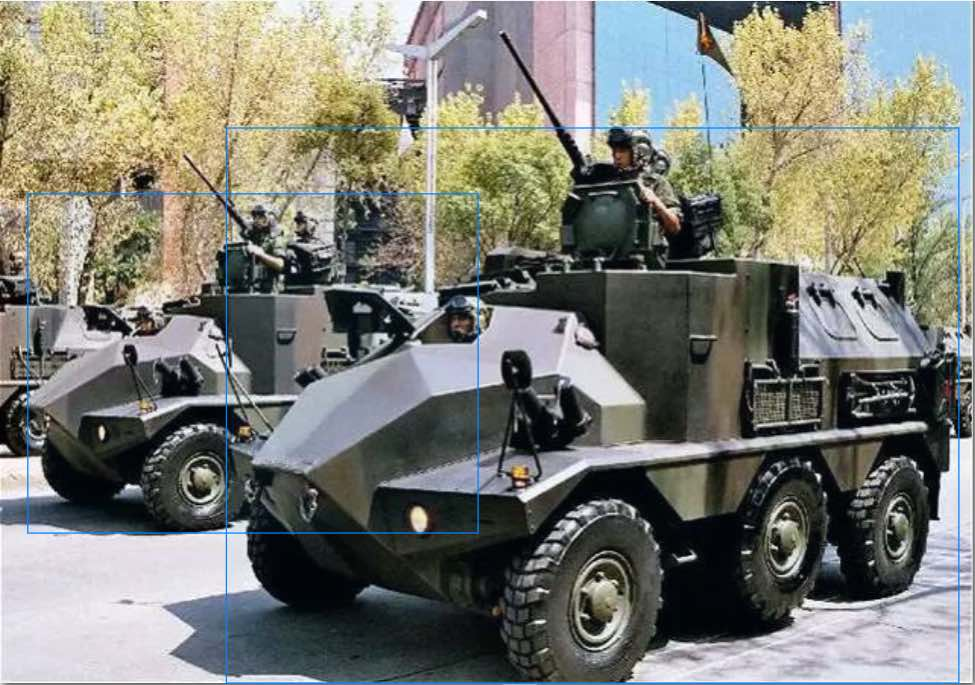
\includegraphics[width=\textwidth]{./images/apc.png}
        \caption{\textbf{APC} - Panhard VCR}
        \label{fig:apc}
    \end{subfigure}
    \vskip\baselineskip
    \begin{subfigure}[b]{0.45\textwidth}
        \centering
        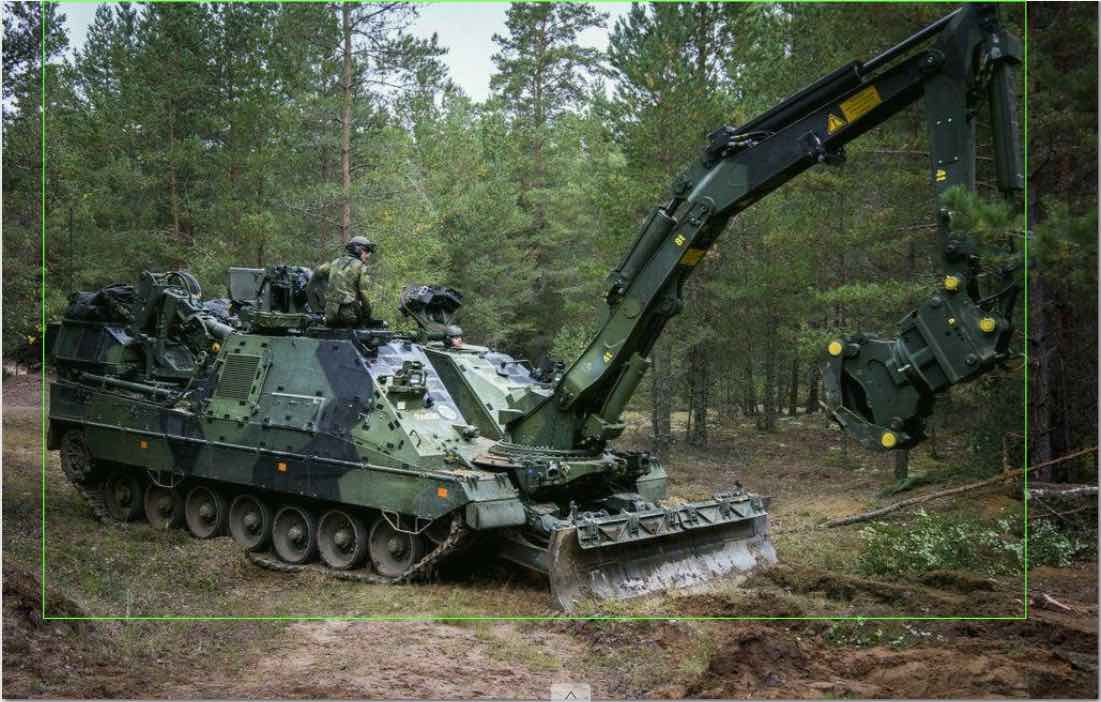
\includegraphics[width=\textwidth]{./images/mev.png}
        \caption{\textbf{MEV} - Kodiak Wisent}
        \label{fig:mev}
    \end{subfigure}
    \hfill
    \begin{subfigure}[b]{0.45\textwidth}
        \centering
        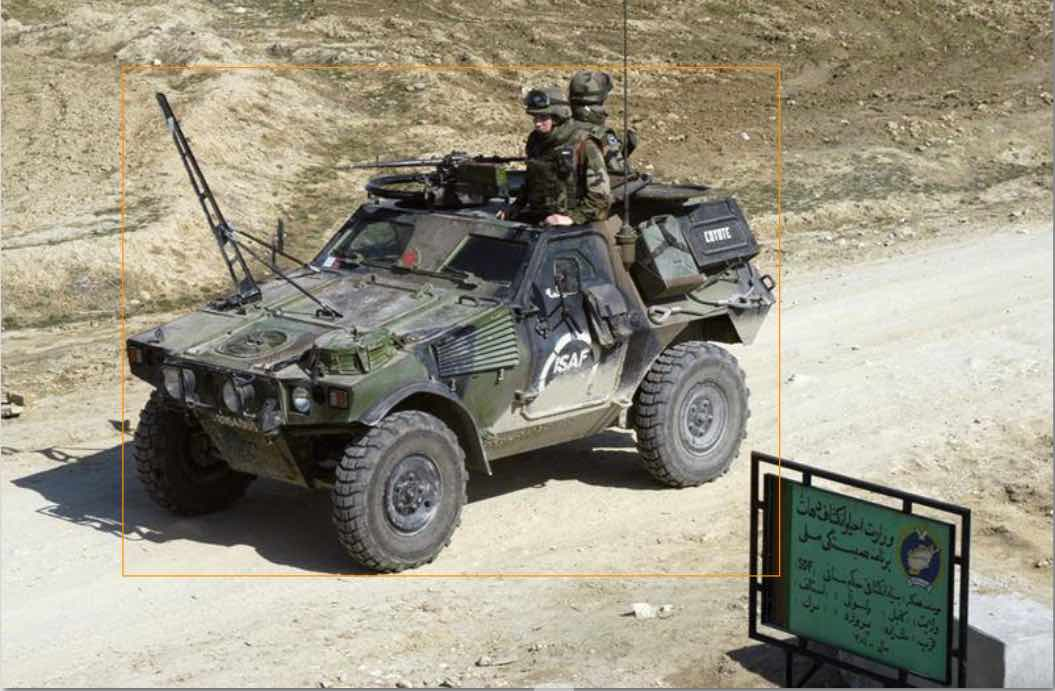
\includegraphics[width=\textwidth]{./images/lav.png}
        \caption{\textbf{LAV} - Panhard VBL}
        \label{fig:lav}
    \end{subfigure}
    \caption{Exemples de véhicules militaires}
    \label{fig:military-vehicles}
\end{figure}


\subsection{Jeu de données d’entraînement}

Nous avons identifié des sources de jeux de données et images  utilisés pour l’entraînement d’algorithmes de visualisation, et des images open source sur Internet.

Nous décrivons dans cette section les jeux de données identifiés et utilisés pour l’entraînement de l’algorithme YoloV8 de détection.

\subsubsection{Open Images v7}

Open Images \cite{openimages2024} est un jeu de données d’environ 9 million d’images annotées, avec notamment 16 million d’annotations bounding boxes pour 600 classes.
Parmi ces classes, une classe Tank contient \textbf{1248 images annotées de véhicules militaires}.

\begin{figure}[H]
    \center
    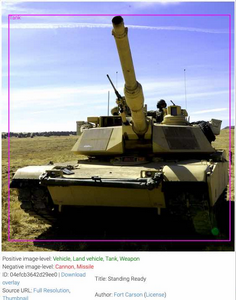
\includegraphics[width=0.4\textwidth]{./images/char-leclerc-openv7.png}
    \caption[Image annotée d’un char]{Image annotée d’un char, extraite du jeu de données Open Images v7.}\label{fig:image-annotée-char}
\end{figure}

\subsubsection{ImageNet}

Le jeu de données ImageNet, créé pour le challenge de détection ILSVRC2012 \cite{imagenet2012}, a été au centre des avancées récentes dans le domaine de la reconnaissance automatique d’objets dans des images par deep-learning.
Ce jeu de données sert aujourd’hui de jeu de données standard pour l’entraînement d’algorithmes de transfert learning.
Il contient plus de 14 million d’images annotées, divisées en 21841 classes.

Parmi ces 21841 classes, plusieurs peuvent contenir des images pertinentes pour la reconnaissance de véhicules militaires. Par exemple, les classes

\begin{itemize}
    \item n02739889 (armored car, armoured car),
    \item n02740061 (armored car, armoured car),
    \item n02740300 (armored personnel carrier, armoured personnel carrier, APC),
    \item n02740533 (armored vehicle, armoured vehicle),
    \item n04389033 (tank, army tank, armored combat vehicle, armoured combat vehicle).
\end{itemize}

Néanmoins, parmi celles-ci seules les images de la classe n04389033 (tank, army tank, armored combat vehicle, armoured combat vehicle) contiennent des annotations pour la détection d’objets.
Cette classe contient \textbf{378 images annotées de véhicules militaires}.

\subsubsection{Roboflow}

Nous disposons désormais de 1624 images annotées de tank, mais cela reste insuffisant pour un entraînement optimal du modèle. Pour obtenir encore plus d'images d'entraînement, nous avons charger un autre dataset annotées de véhicules militaires, mis à disposition par \textit{Tuomo Hiippala du Digital Geography Lab}.\cite{roboflow2024}
Ce jeu de données contient \textbf{1042 images} dont 89 images négatives avec 10 classes (bm-21, t-80, t-64, t-72, bmp-1, bmp-2, bmd-2, btr-70, btr-80 et mt-lb) que nous avons par la suite mapper en AFV (tank).


\subsubsection{Données disponibles librement}

Une recherche d’images sur Internet permet de trouver aisément des exemples pouvant servir à l’entraînement d’un algorithme de détection de véhicules. (Google)
Plusieurs facteurs sont cependant à prendre en compte.


\begin{itemize}
    \item Premièrement, les images que l’on peut trouver ne sont pas annotées, et demandent donc un travail supplémentaire d’annotation manuelle.
          \begin{figure}[H]
              \center
              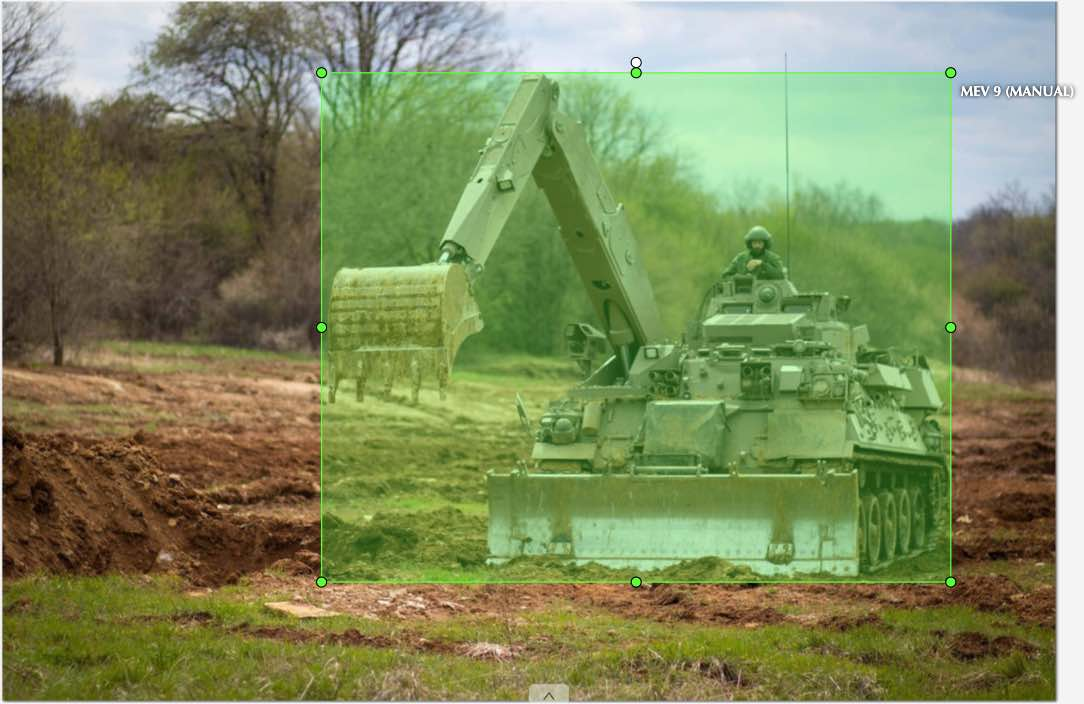
\includegraphics[width=0.5\textwidth]{./images/anotation-manuelle.png}
              \caption{Annotation manuelle d’une image d’engin blindé du génie.}\label{fig:anotation-manuelle}
          \end{figure}
    \item Deuxièmement, ces images servent principalement à répondre aux attentes des utilisateurs d’un moteur de recherche, et ne correspondent pas nécessairement aux critères attendus pour l’entraînement d’un algorithme de détection d’objets.
          Ainsi, une recherche d’images de char Leclerc donnera des résultats qui présentent l’objet en gros plan, clairement identifiable.
          Il est difficile d’obtenir des images qui présentent l’objet « en situation réelle de combat », ce qui limitera la qualité du modèle entraîné.
\end{itemize}

Nous avons tout de même pu constituer, à partir d’une recherche limitée pour certains modèles de véhicules militaires, un premier corpus composé de \textbf{669 images}. Nous avons annoté manuellement ces 669 images avec quatre classes.\\


\subsubsection{Etapes de la collecte des images}

Nous avons reparti la collecte en deux grandes étapes:\\

\indent \textbf{Prepare-01 :} Nous commençons par créer un jeu de données d'entraînement à partir des données disponibles librement sur Internet. (ImageNet, OpenImages, Roboflow).

\noindent Pour cette première étape, nous avons collecté \textbf{2666 images} de véhicules militaires dont \textbf{2577 images positives} et \textbf{89 images négatives}.
A cette étape, nous avons travaillé avec une classe \textbf{tank}.\\


\textbf{Prepare-02 :} Nous utilisons également des outils de scraping pour collecter davantage d'images de véhicules militaires à partir d'images Google.

\noindent Nous avons collectés 669 images de plus, ce qui nous fait un total de \textbf{3335 images de véhicules}. (Figure \ref{fig:fiftyone-dataset})

Ce nombre d'images nous permet de définir quatre grandes classes (AFV, APC, MEV et LAV) de véhicules militaires que notre modèle peut ensuite discriminer.


\begin{figure}[H]
    \center
    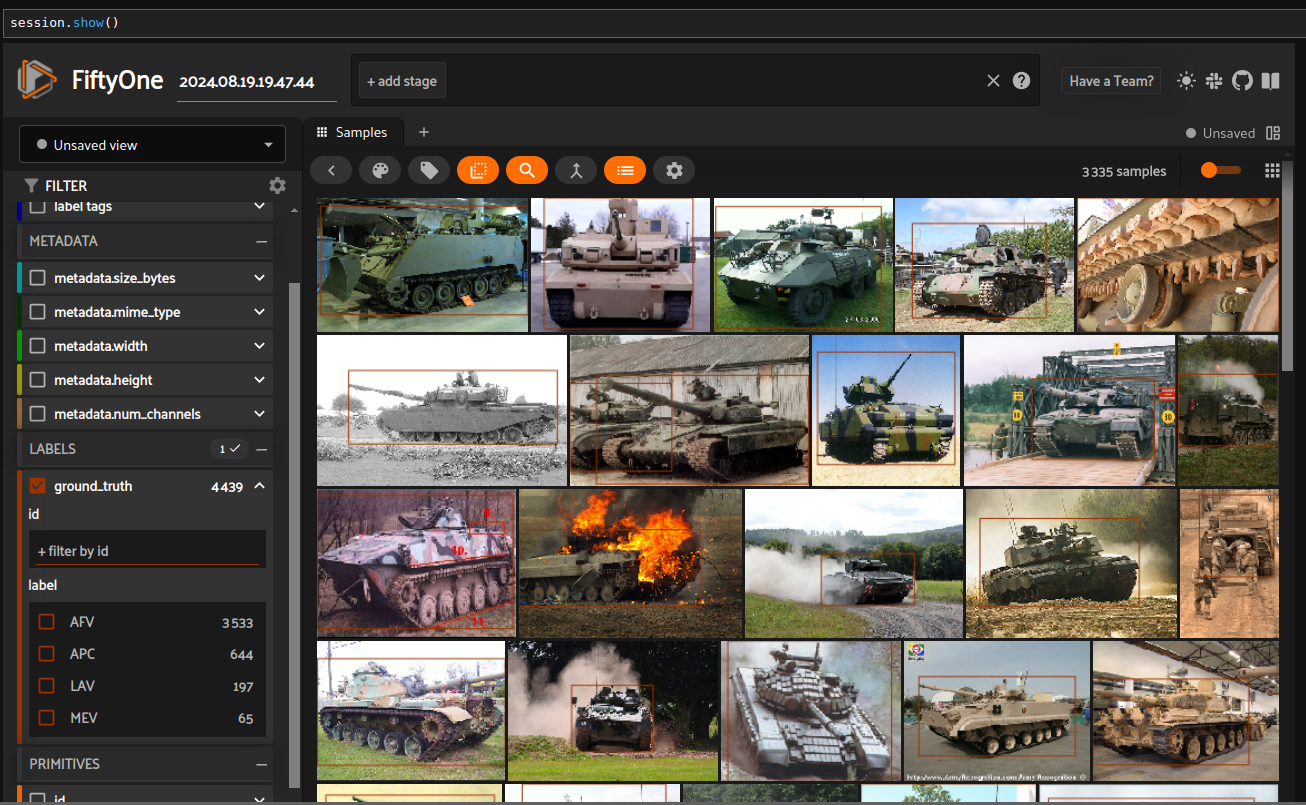
\includegraphics[width=0.8\textwidth]{./images/fiftyone-dataset.png}
    \caption[Fiftyone dataset]{FiftyOne - Jeu de données (3335 images)}\label{fig:fiftyone-dataset}
\end{figure}


\section{Résultats des premiers entraînements}

A ce niveau de l'expérience, la collecte des données du dataset d'entraînement c'est faite en deux grandes étapes (Prepare-01 et Prepare-02).
Nous allons présenter les résultats d'entraînement avec images positives et négatives sur les différentes tailles du modèles YoloV8.
Les images positives sont celles qui contiennent un ou plusieurs des objets définis (i.e. Tank, Camion militaire, Char militaire, ...).
Les images négatives sont celles qui contiennent autre chose que les objets définis.\\

La précision (\textbf{mAP : Mean Average Precision}) de notre modèle sera relevée à la fin de chaque entraînement afin de suivre son évolution.

\begin{equation}
    \mathrm{mAP} = \frac{1}{N} \sum_{i=1}^{N} \mathrm{AP}_i
\end{equation}

\begin{itemize}
    \item \textbf{N} : Représente le nombre total de classes dans le dataset.
    \item \textbf{AP$_i$} : Représente l'Average Precision (Précision Moyenne) pour la $i$-ème classe.
    \item \textbf{mAP} : Représente la moyenne des précisions moyennes sur toutes les classes.
\end{itemize}



\subsection*{Prepare-01: ImageNet, OpenImages, Roboflow (2666 images)}
\label{results-prepare01}


A cette étape, le modèle détecte uniquement une classe 'tank', donc la mAP sera une moyenne de toutes les images.

Nous avons essayé plusieurs scénarios sur l’algorithme en changeant le paramètres \textit{Epoch} (époques: passe complète à travers toutes les instances de dataset d'entraînement.) et la taille du modèles.

\newcolumntype{C}[1]{>{\centering\arraybackslash}p{#1}}


\begin{table}[H]
    \centering
    \begin{tabular}{|C{2cm}|C{4cm}|C{2cm}|C{2cm}|}
        \hline
        \textbf{Modèle} & \textbf{Images négatives} & \textbf{Epoch} & \textbf{mAP} \\ \hline
        \multirow{3}{*}{yolov8m}
                        & \multirow{3}{*}{Oui}      & 60             & 0.6606       \\ \cline{3-4}
                        &                           & 80             & 0.6548       \\ \cline{3-4}
                        &                           & 100            & 0.6476       \\ \cline{2-4}
                        & \multirow{4}{*}{Non}      & 60             & 0.7137       \\ \cline{3-4}
                        &                           & 70             & 0.6920       \\ \cline{3-4}
                        &                           & 80             & 0.7000       \\ \cline{3-4}
                        &                           & 100            & 0.7000       \\ \hline
        \multirow{3}{*}{yolov8l}
                        & \multirow{3}{*}{Oui}      & 60             & 0.6512       \\ \cline{3-4}
                        &                           & 80             & 0.6491       \\ \cline{3-4}
                        &                           & 100            & 0.6384       \\ \hline
        \multirow{3}{*}{yolov8x}
                        & \multirow{3}{*}{Oui}      & 60             & 0.6518       \\ \cline{3-4}
                        &                           & 80             & 0.6535       \\ \cline{3-4}
                        &                           & 100            & 0.6308       \\ \hline
    \end{tabular}
    \caption{Résultats des entraînements à l’étape Prepare-01 (2666 images)}
    \label{tab:train-prepare01}
\end{table}




Au vu de ces résultats, nous nous sommes rendu compte que la taille du modèle n'influence pas les résultats. Nous allons donc uniquement travailler avec la taille medium du modèle YoloV8.
Nous allons également utiliser des datasets contenant des images annotées.


\subsection*{Prepare-02: ImageNet, OpenImages, Roboflow and Google  (3335 images)}
\label{results-prepare02}

A cette étape, nous avons entraîné le modèle a détecter les 04 classes (AFV, APC, MEV, LAV).
La moyenne mAP tient donc compte de ces 04 classes, mais nous allons aussi fournir la moyenne de chacune des classes.

\textbf{yolov8m :}  Epoch = 60 $\Rightarrow$ mAP = 0.6609276140054803

\begin{table}[H]
    \centering
    \begin{tabular}{|c|c|c|c|c|}
        \hline
        \textbf{Classes} & \textbf{Précision} & \textbf{Recall} & \textbf{F1-score} & \textbf{Support} \\ \hline
        AFV              & 0.76               & 0.85            & 0.80              & 343              \\ \hline
        APC              & 0.69               & 0.72            & 0.70              & 64               \\ \hline
        LAV              & 0.55               & 0.72            & 0.62              & 25               \\ \hline
        MEV              & 0.62               & 0.71            & 0.67              & 7                \\ \hline
        micro avg        & 0.74               & 0.82            & 0.78              & 439              \\ \hline
        macro avg        & 0.65               & 0.75            & 0.70              & 439              \\ \hline
        weighted avg     & 0.74               & 0.82            & 0.78              & 439              \\ \hline
    \end{tabular}
    \caption{Résultats des entraînements à l'étape Prepare-02 (3335 images)}
    \label{tab:map-train-01}
\end{table}




\section{Tracking}

Après avoir entraîné notre model avec notre jeu de donnée, nous utilisons le meilleur model (\textbf{best.pt}) obtenu pendant l'entraînement et un tracker (\textbf{botsort.yaml}) pour tracker les objets dans les vidéos.


\begin{figure}[H]
    \center
    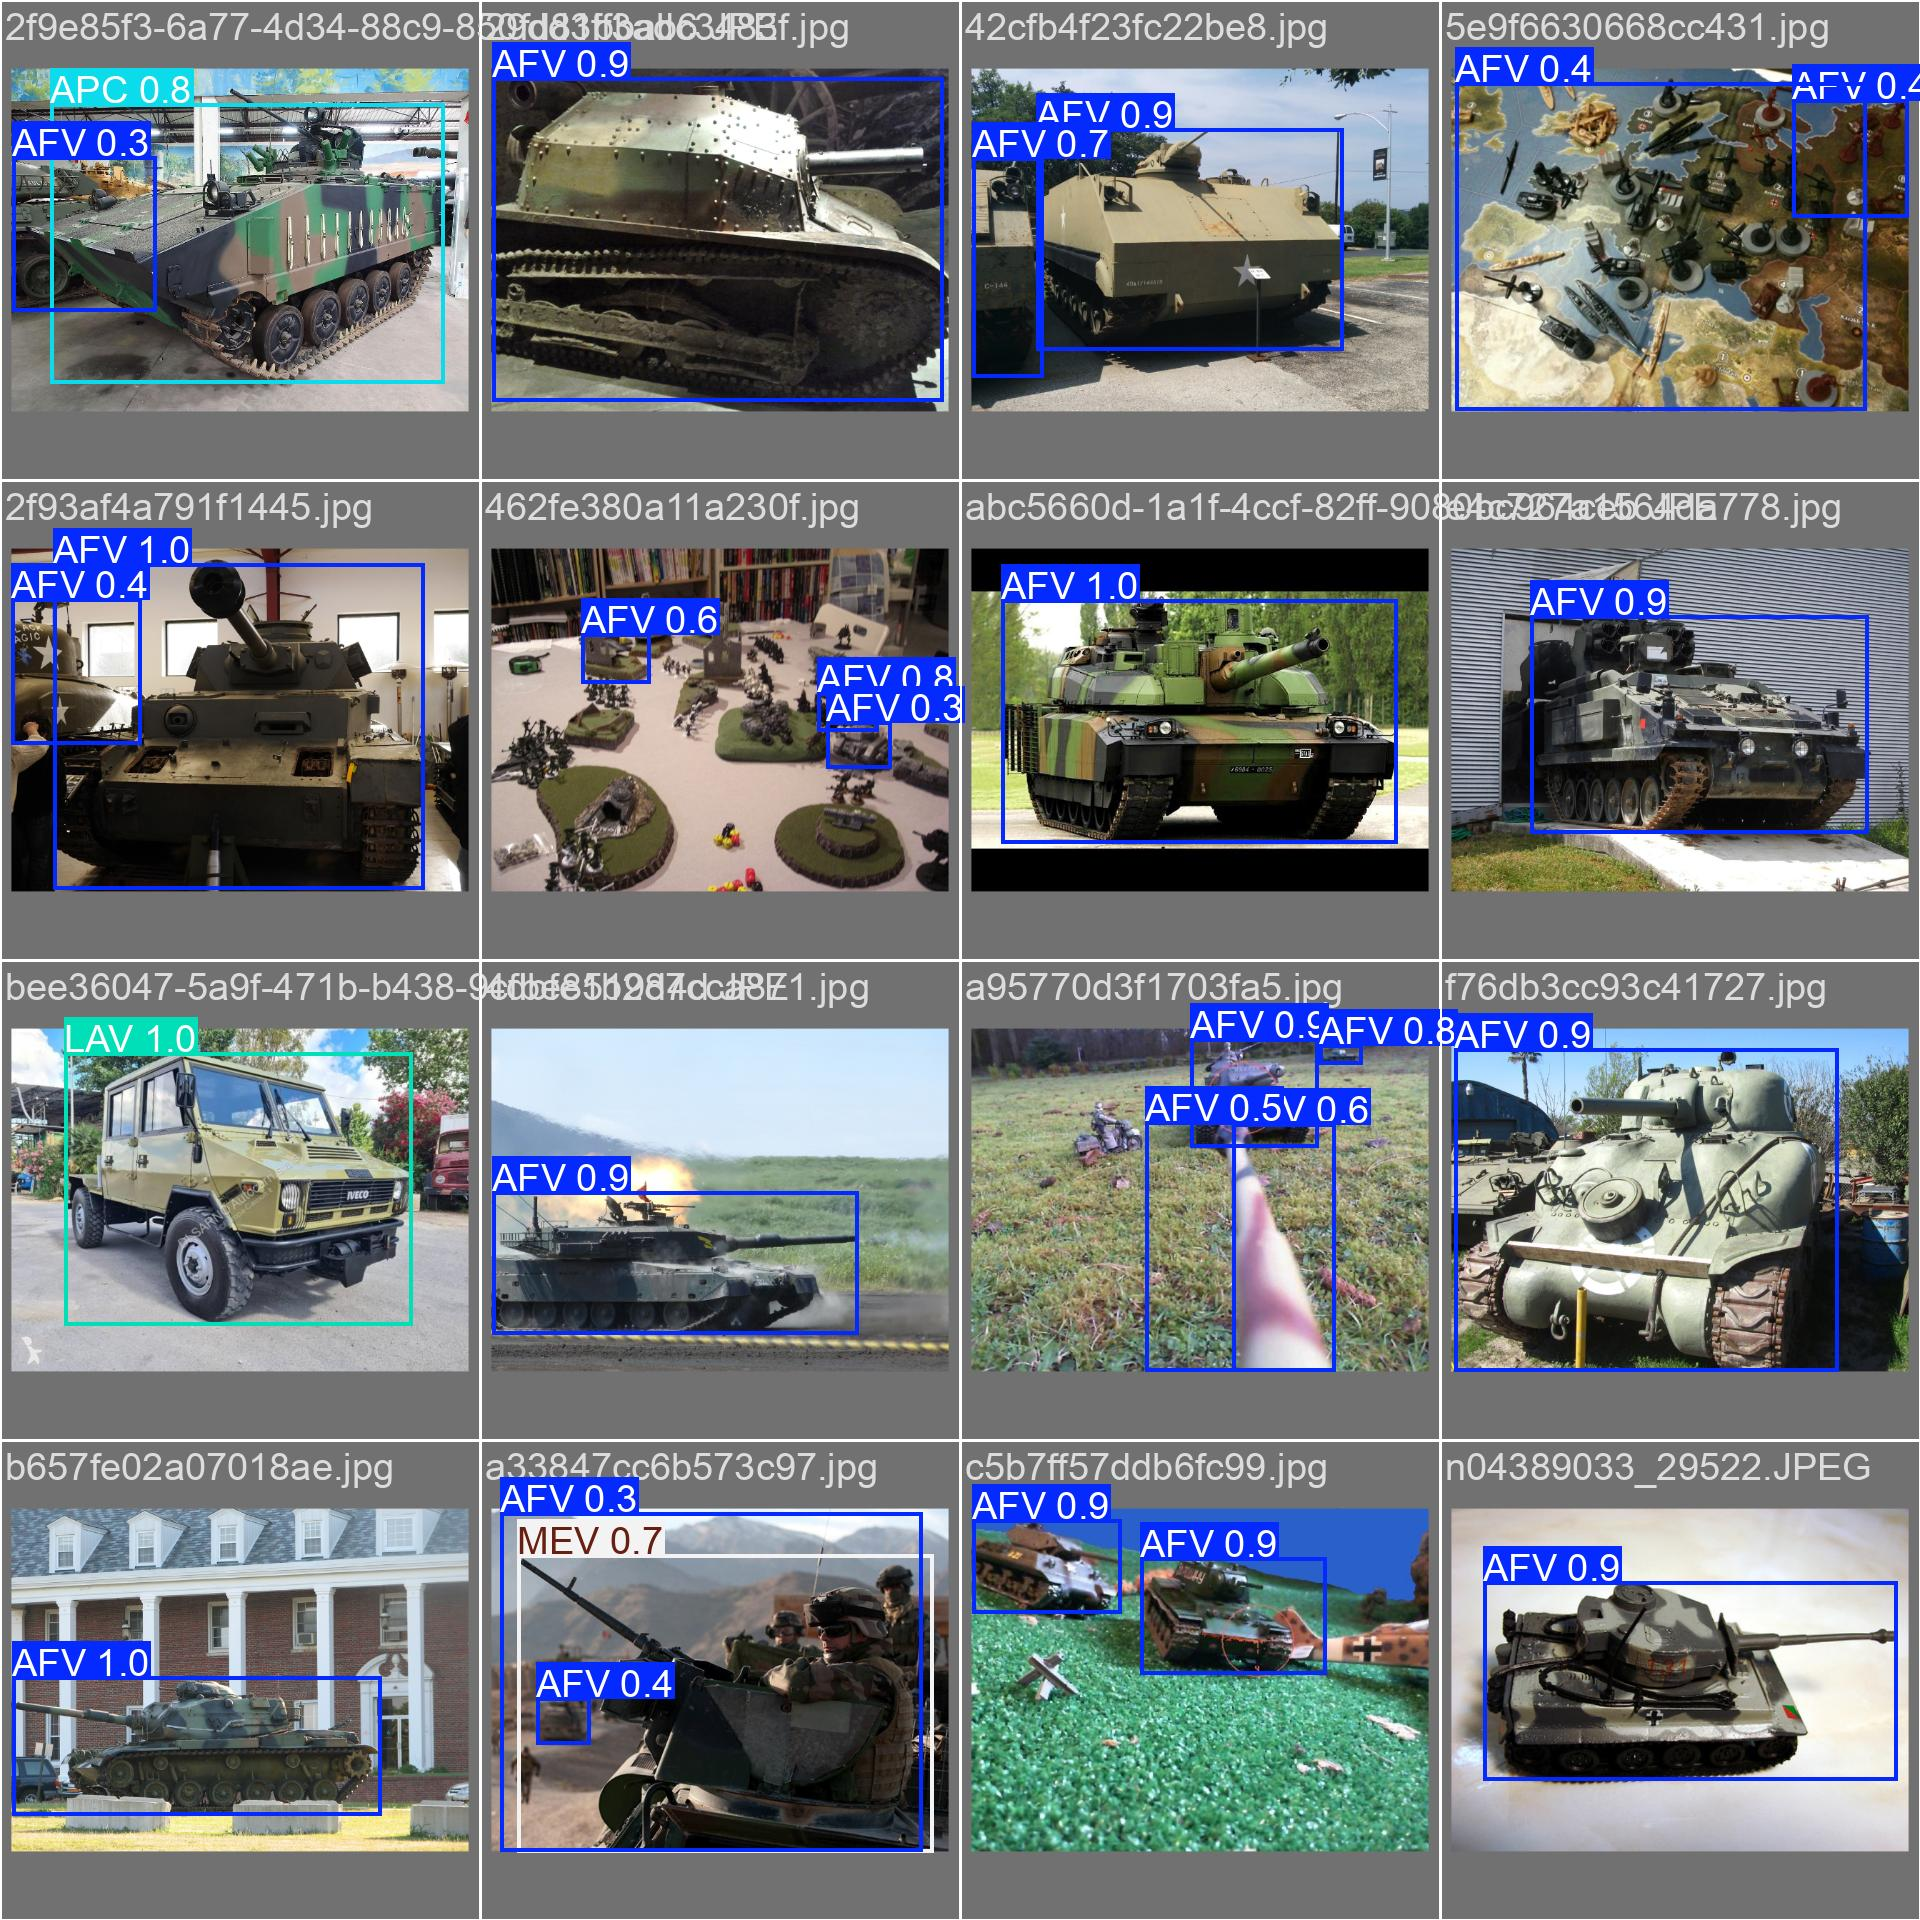
\includegraphics[width=0.6\textwidth]{./images/track2_val.jpg}
    \caption[Détection et reconnaissance avec taux de précision]{Détection et reconnaissance avec taux de précision}\label{fig:track2_val}
\end{figure}


\section{Augmentation des données}

\subsection{Images transformées}

Nous avons utilisé des méthodes d'augmentation des données afin d'améliorer la capacité du modèle à reconnaître des véhicules même lorsqu'ils sont éloignés ou partiellement masqués. Les méthodes utilisées incluent :

\begin{itemize}
    \item Une transformation \textbf{scale} pour dézoomer l'image et donner l'impression que le véhicule est vu de loin. (Figure \ref{fig:scale_transformed})
    \item Une transformation \textbf{XYMasking} pour masquer des bandes horizontales ou verticales, simulant un véhicule caché par un obstacle. (Figure \ref{fig:xymasking})
    \item Une transformation de type \textbf{Météo} pour donner l'impression qu'il y a de la neige, de la pluie ou du brouillard sur l'image. (Figure \ref{fig:meteo})
\end{itemize}


\begin{figure}[H]
    \centering
    \begin{subfigure}[b]{0.45\textwidth}
        \centering
        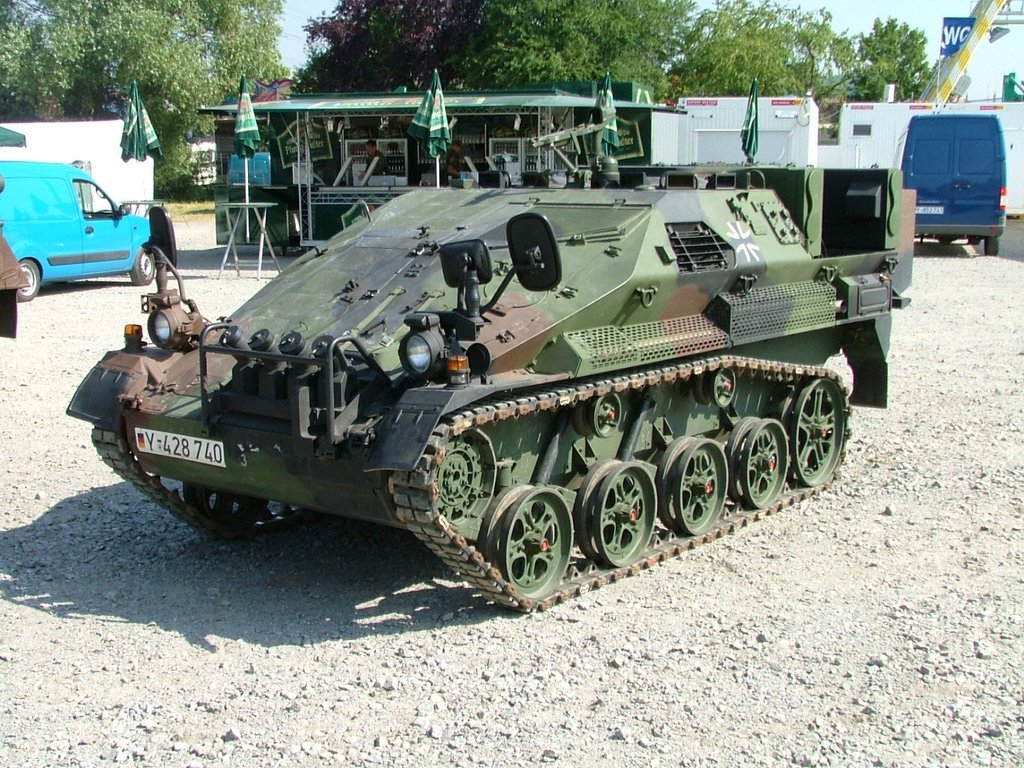
\includegraphics[width=\textwidth]{./images/original-image.jpg}
        \caption{Image originale}
        \label{fig:original-image}
    \end{subfigure}
    \hfill
    \begin{subfigure}[b]{0.45\textwidth}
        \centering
        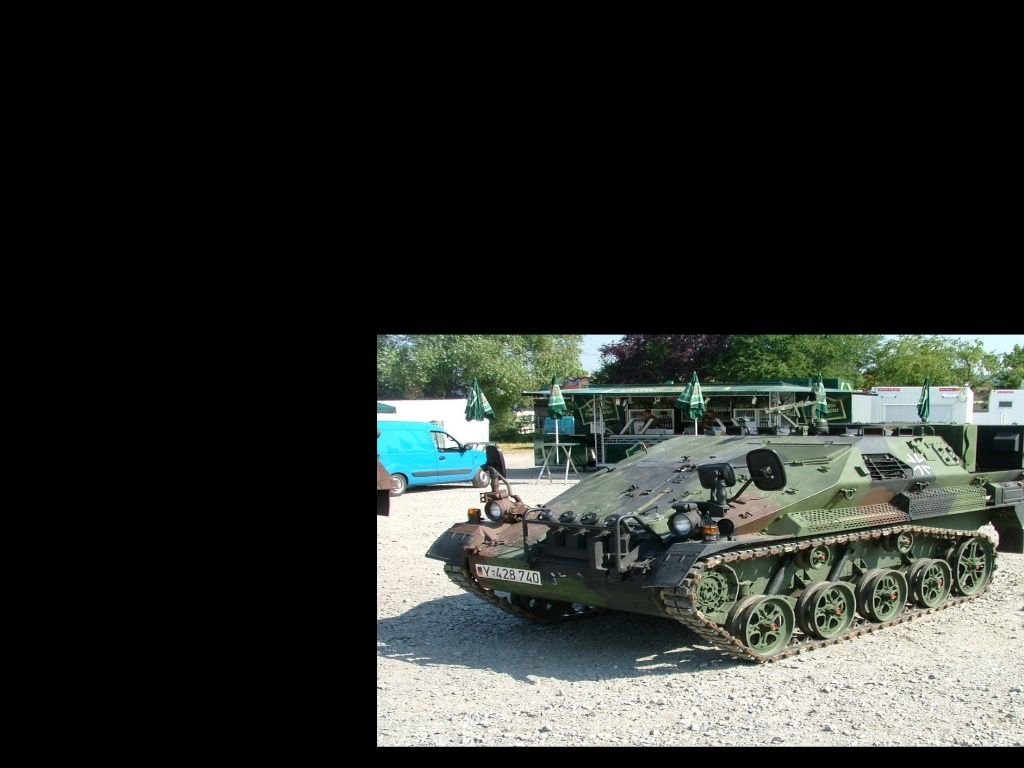
\includegraphics[width=\textwidth]{./images/scale_transformed.jpg}
        \caption{Effet zoom}
        \label{fig:scale_transformed}
    \end{subfigure}
    \vskip\baselineskip
    \begin{subfigure}[b]{0.45\textwidth}
        \centering
        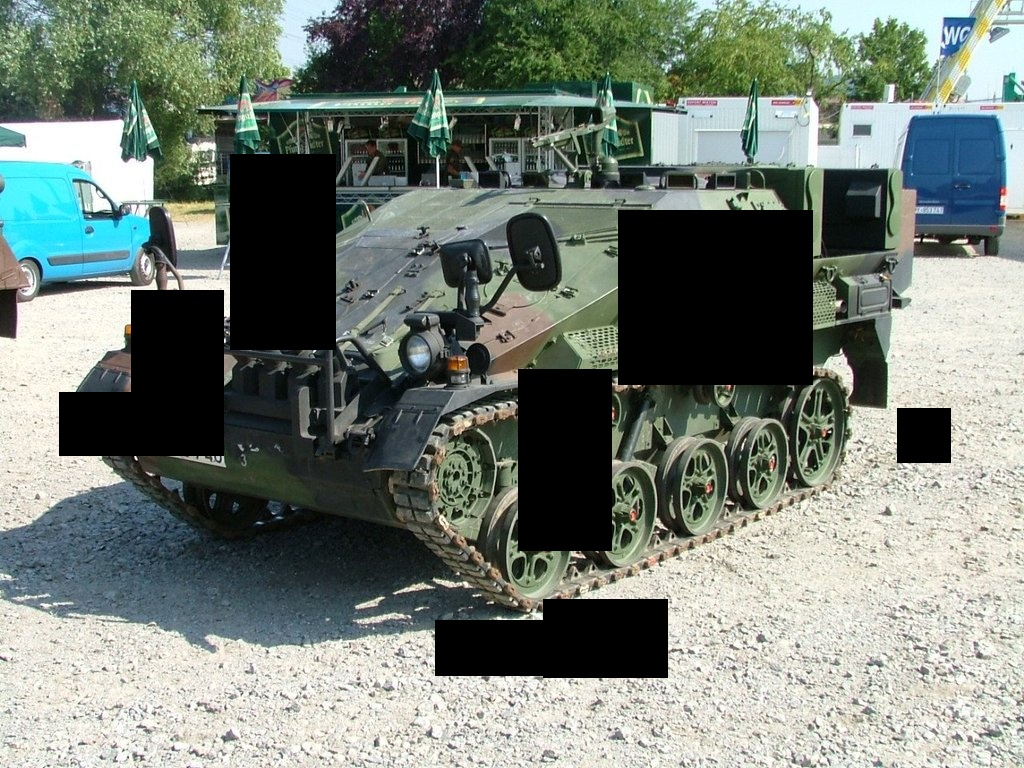
\includegraphics[width=\textwidth]{./images/xymasking.jpg}
        \caption{XYMasking}
        \label{fig:xymasking}
    \end{subfigure}
    \hfill
    \begin{subfigure}[b]{0.45\textwidth}
        \centering
        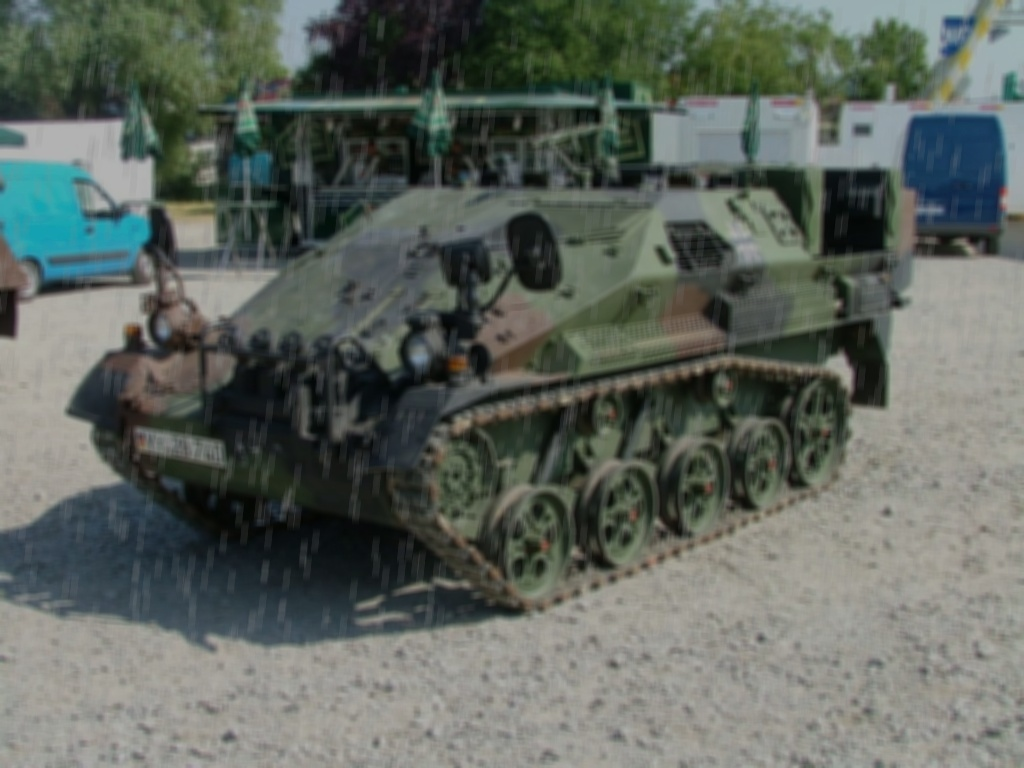
\includegraphics[width=\textwidth]{./images/weather_effect.jpg}
        \caption{Météo (pluie)}
        \label{fig:meteo}
    \end{subfigure}
    \caption{Exemples transformation d'images de véhicules militaires}
    \label{fig:military-vehicles}
\end{figure}




\noindent Les étapes spécifiques suivies sont les suivantes :

\begin{enumerate}
    \item Dans un premier temps, nous avons récupéré une image de notre dataset avec ses labels (bounding boxes).
    \item Puis, nous avons créé une fonction qui applique les trois transformations à toutes les images du dataset.
    \item Enfin, nous avons entraîné le modèle YOLO avec ce dataset augmenté.
\end{enumerate}

Après l'augmentation des images, nous avons pu collecter en plus du dataset existant, \textbf{8403 images}.\\


\subsubsection{Résultats des entraînements du modèle (Etape Prepare-03) }
\label{results-prepare03}

Nous avons entraîné notre modèles avec tous les jeux de données :
\textbf{Dataset ImageNet, OpenImages, Roboflow, Google et images transformées}, pour un total de 8403 images de véhicules militaires.

\textbf{yolov8m :}
Epoch = 60 $\Rightarrow$ mAP = 0.34253746508577226

\begin{table}[H]
    \centering
    \begin{tabular}{|c|c|c|c|c|}
        \hline
        \textbf{Classe} & \textbf{Précision} & \textbf{Recall} & \textbf{F1-score} & \textbf{Support} \\ \hline
        AFV             & 0.71               & 0.66            & 0.68              & 731              \\ \hline
        APC             & 0.59               & 0.57            & 0.58              & 100              \\ \hline
        LAV             & 0.51               & 0.41            & 0.46              & 56               \\ \hline
        MEV             & 0.22               & 0.40            & 0.29              & 10               \\ \hline
        micro avg       & 0.68               & 0.63            & 0.65              & 897              \\ \hline
        macro avg       & 0.51               & 0.51            & 0.50              & 897              \\ \hline
        weighted avg    & 0.68               & 0.63            & 0.65              & 897              \\ \hline
    \end{tabular}
    \caption{Résultats des entraînements à l'étape Prepare-03 (8403 images)}
    \label{tab:results_moy_prepare03}
\end{table}

\subsubsection{Moyenne des résultats des entraînements du modèle (Etape Prepare-03).}

Nous avons quand tenu à faire des entraînements en testant encore les différentes versions du modèle yolov8 et les valeurs d'époques.
Ci dessous, une synthèse des results:

\begin{table}[H]
    \centering
    \begin{tabular}{|c|c|c|c|c|c|c|c|}
        \hline
        \multirow{2}{*}{\textbf{Modèles}} & \multirow{2}{*}{\textbf{Epoch}} & \multirow{2}{*}{\textbf{mAP}} & \multicolumn{4}{c|}{\textbf{Précision par classe}} & \multirow{2}{*}{\textbf{micro avg}}                      \\ \cline{4-7}

                                          &                                 &                               & AFV                                                & APC                                 & LAV  & MEV  &      \\ \hline
        \multirow{5}{*}{\texttt{yolov8m}}
                                          & 60                              & 0.343                         & 0.71                                               & 0.59                                & 0.51 & 0.22 & 0.68 \\ \cline{2-8}
                                          & 70                              & 0.364                         & 0.71                                               & 0.57                                & 0.51 & 0.26 & 0.67 \\ \cline{2-8}
                                          & 80                              & 0.405                         & 0.73                                               & 0.54                                & 0.51 & 0.21 & 0.67 \\ \cline{2-8}
                                          & 90                              & 0.374                         & 0.72                                               & 0.63                                & 0.49 & 0.26 & 0.69 \\ \cline{2-8}
                                          & 100                             & 0.327                         & 0.67                                               & 0.49                                & 0.60 & 0.27 & 0.64 \\ \hline
        \multirow{2}{*}{\texttt{yolov8l}}
                                          & 80                              & 0.360                         & 0.69                                               & 0.53                                & 0.45 & 0.24 & 0.65 \\ \cline{2-8}
                                          & 100                             & 0.331                         & 0.69                                               & 0.63                                & 0.52 & 0.21 & 0.67 \\ \hline
    \end{tabular}
    \caption{Moyenne des résultats des entraînements à l'étape Prepare-03 (8403 images).}
    \label{tab:results-moy-prepare03}
\end{table}




\subsection{Images synthétiques}

Dans cette partie de travail nous allons générer des images synthétiques.

Pour cette expérience, nous avons utilisé Dreambooth \cite{ruiz2023dreambooth} pour générer des images de véhicules militaires afin d'entraîner notre modèle de détection de véhicules.
Notre modèle souffre d'un manque de diversité dans ses données d'entraînement disponibles, nous avons essayé améliorer notre jeu de données d'entraînement avec des images synthétiques générées par un modèle texte-image.
Dreambooth est une méthode permettant de personnaliser les modèles texte-image avec seulement quelques images d'un sujet.
DreamBooth est utilisé pour finetuner les différentes versions du modèle \textbf{Stable Diffusion} \cite{rombach2021highresolution}.\\



\subsubsection{Finetuning du modèle}

Pour l'entrainement du modèle, nous avons de lui fournir un échantillon d'image du véhicule qu'on souhaite généré.
Dans notre cas, nous avons utilisé \textbf{200 images de char Leclerc}.
Nous entraînons avec LoRA, sur 800 étapes, en enregistrant les points de contrôle toutes les 250 étapes.\\

Nous avons ci dessous notre script qui permet d'entrainer notre model de diffusion :

\lstset{style=mystyle}

\begin{lstlisting}[language=Python, basicstyle=\footnotesize\ttfamily, breaklines=false]
!accelerate launch ../diffusers/examples/dreambooth/train_dreambooth_lora_sdxl.py \
    --pretrained_model_name_or_path="stabilityai/stable-diffusion-xl-base-1.0" \
    --pretrained_vae_model_name_or_path="madebyollin/sdxl-vae-fp16-fix" \
    --train_text_encoder \
    --instance_data_dir="../resources/leclerc" \
    --class_data_dir="../tanks" \
    --output_dir="./adomvi-dream-tank-xl_1024" \
    --mixed_precision="fp16" \
    --with_prior_preservation --prior_loss_weight=1.0 \
    --instance_prompt="a photo of [L] tank" \
    --class_prompt="a photo of a tank" \
    --num_class_images=400 \
    --resolution=1024 \
    --train_batch_size=1 \
    --use_8bit_adam \
    --enable_xformers_memory_efficient_attention \
    --gradient_accumulation_steps=1 \
    --checkpointing_steps=250 \
    --learning_rate=5e-5 \
    --lr_scheduler="constant" \
    --lr_warmup_steps=0 \
    --max_train_steps=800 \
    --validation_prompt="A photo of [L] tank on the moon" \
    --validation_epochs=50 \
    --seed="0"
\end{lstlisting}

Dans ce cas nous avons utilisé la version XL de stable diffusion comme modèle de base. Nous avons fait plusieurs tests sur les autres versions.

\begin{table}[H]
    \centering
    \begin{tabular}{|p{3cm}|p{4cm}|p{7cm}|}
        \hline
        \textbf{Version} & \textbf{Taille recommandée des images à générer} & \textbf{Licence d'utilisation}                      \\ \hline
        1.5              & 512 x 512 pixels                                 & CreativeML OpenRAIL M license                       \\ \hline
        2.0              & 768 x 768 pixels                                 & CreativeML OpenRAIL M license                       \\ \hline
        SDXL base 1.0    & 1024 x 1024 pixels                               & CreativeML OpenRAIL ++-M License                    \\ \hline
        3.0              & 1024 x 1024 pixels                               & Stability Non-Commercial Research Community License \\ \hline
    \end{tabular}
    \caption{Comparaison des versions de modèles de stable diffusion.\cite{wiki:stable_diffusion}}
    \label{tab:modeles}
\end{table}



\subsubsection{Génération d'images}

Une fois notre modèle entrainé, nous pouvons exécuter des inférences pour générer de nouvelles images d'un char Leclerc.
Étant donné que notre jeu de données de véhicules militaires d'origine ne contient pas d'images prises à distance ou dans lesquelles le sujet est partiellement caché, nous avons générer de telles images en redigant des prompts complexes.\\

Ci-dessous nous avons un extrait de script permettant de générer les images:
\begin{lstlisting}[language=Python, basicstyle=\footnotesize\ttfamily, breaklines=true]
    lora_model_id = "../adomvi-dream-tank-xl_1024"
    model_base = "stabilityai/stable-diffusion-xl-base-1.0"
    
    prompts = {
        "desert": "[L] tank moving in the desert behind rocks, seen from the top of a distant hill, respecting realistic scale and dimensions",
        "urban_combat": "[L] tank in urban combat, maneuvering between buildings, seen from a high-rise far away, respecting realistic scale and dimensions",
        "forest_camouflage": "[L] tank camouflaged in a dense forest, barely visible among trees, seen from very far away, respecting realistic scale and dimensions",
    }
    
    negative_prompt = "close-up, upfront, unobstructed, bad scale, inaccurate canons, extra canons, out of frame, lowres, text, error, cropped, worst quality, low quality, jpeg artifacts, duplicate, bad proportions, extra elements, malformed structures"
    
    generate_images(
        lora_model_id=lora_model_id,
        model_base=model_base,
        prompts=prompts,
        negative_prompt=negative_prompt,
        inference_dir=inference_dir,
        width = 1024,
        height = 1024,
        num_inference_steps = 150
    )
\end{lstlisting}



\subsubsection{Images générées}

Plusieurs version du modèle Stable Diffusion ont été utilisé durant cette expérience.

\begin{figure}[H]
    \center
    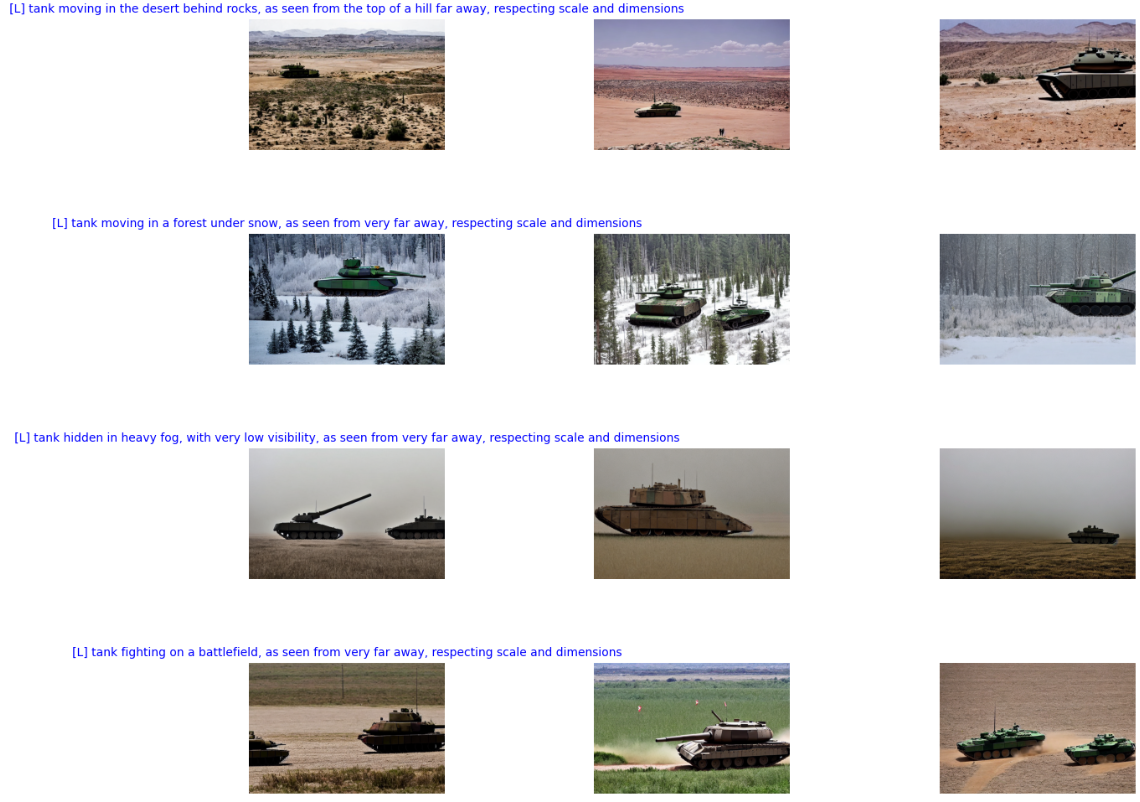
\includegraphics[width=1\textwidth]{./images/v1-5_sd_dreambooth.png}
    \caption{prompts + Images générés avec le modèle stable-diffusion v1.5}
    \label{fig:image_sdv15}
\end{figure}

Tout d'abord, nous avons généré des images avec la version v1.5 de Stable Diffusion.
Arès avoir observé les résultats, nous avons poursuivi nos tests en utilisant une version plus récente du modèle.

\begin{figure}[H]
    \centering
    \begin{subfigure}[b]{0.49\textwidth}
        \centering
        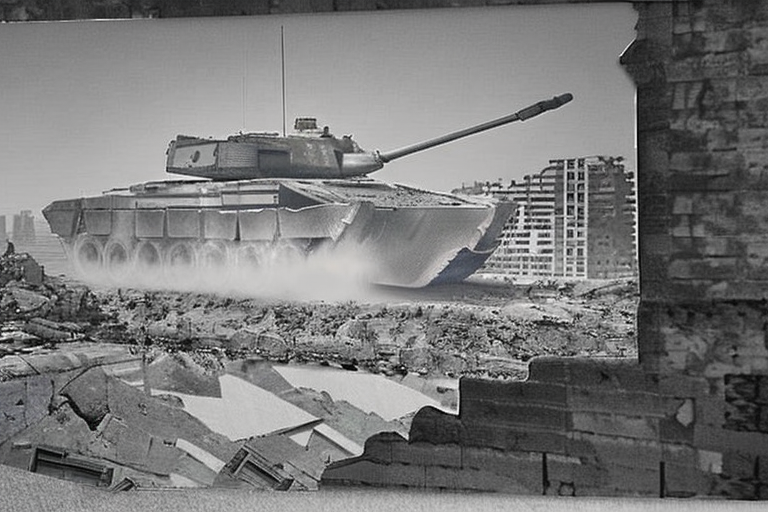
\includegraphics[width=\textwidth]{./images/v2_tank-city_ruins-1.png}
        \caption{Dans les ruines de la ville}
    \end{subfigure}
    \begin{subfigure}[b]{0.49\textwidth}
        \centering
        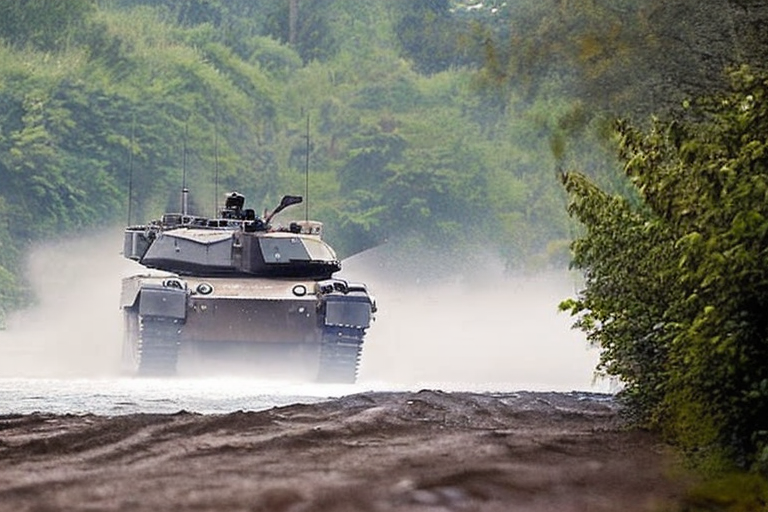
\includegraphics[width=\textwidth]{./images/v2_tank-rainy_day-3.png}
        \caption{Par un jour pluvieux}
    \end{subfigure}
    \hfill
    \begin{subfigure}[b]{0.49\textwidth}
        \centering
        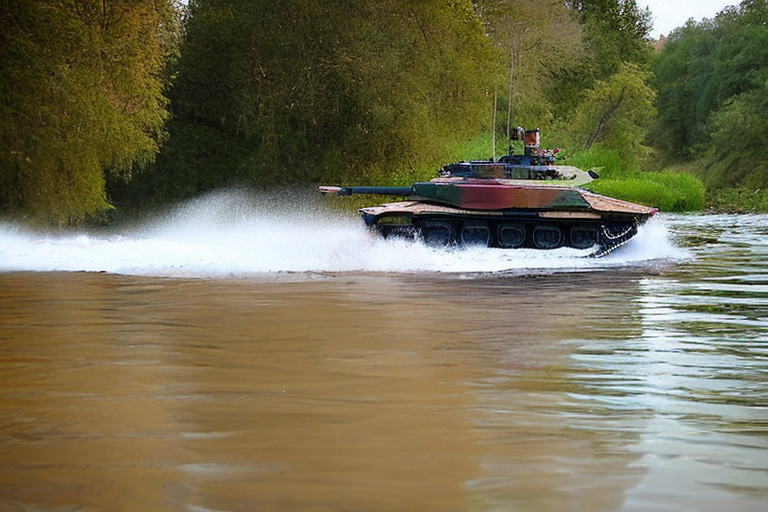
\includegraphics[width=\textwidth]{./images/v2_tank-river_crossing-0.png}
        \caption{Traversée de rivière}
    \end{subfigure}
    \begin{subfigure}[b]{0.49\textwidth}
        \centering
        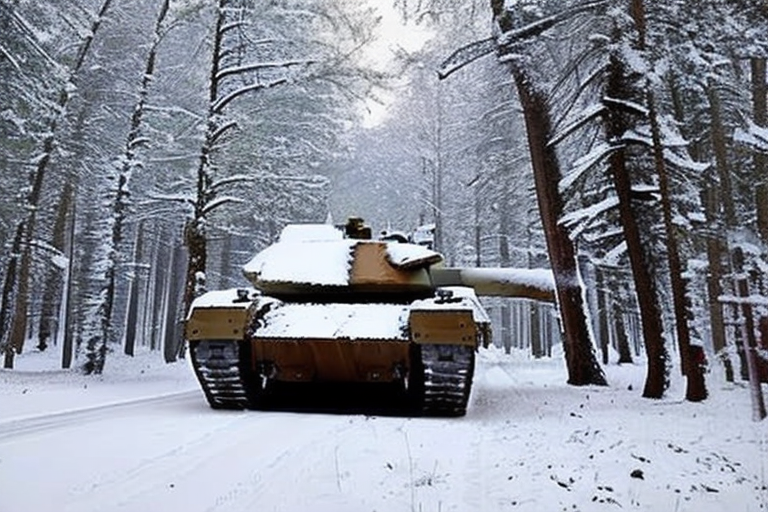
\includegraphics[width=\textwidth]{./images/v2_tank-snow-1.png}
        \caption{Sous la neige}
    \end{subfigure}
    \caption{Images générés avec le modèle stable-diffusion v2}
    \label{fig:image_sdv2}
\end{figure}


Ensuite, nous avons utilisé la version v2 de Stable Diffusion pour générer des images dans différentes conditions météorologiques et contextes.
Nous avons procédé à des expérimentations avec la version XL du modèle Stable-Diffusion, offrant de nouvelles améliorations en termes de détails et de précision des images générées.

\begin{figure}[H]
    \centering
    \begin{subfigure}[b]{0.49\textwidth}
        \centering
        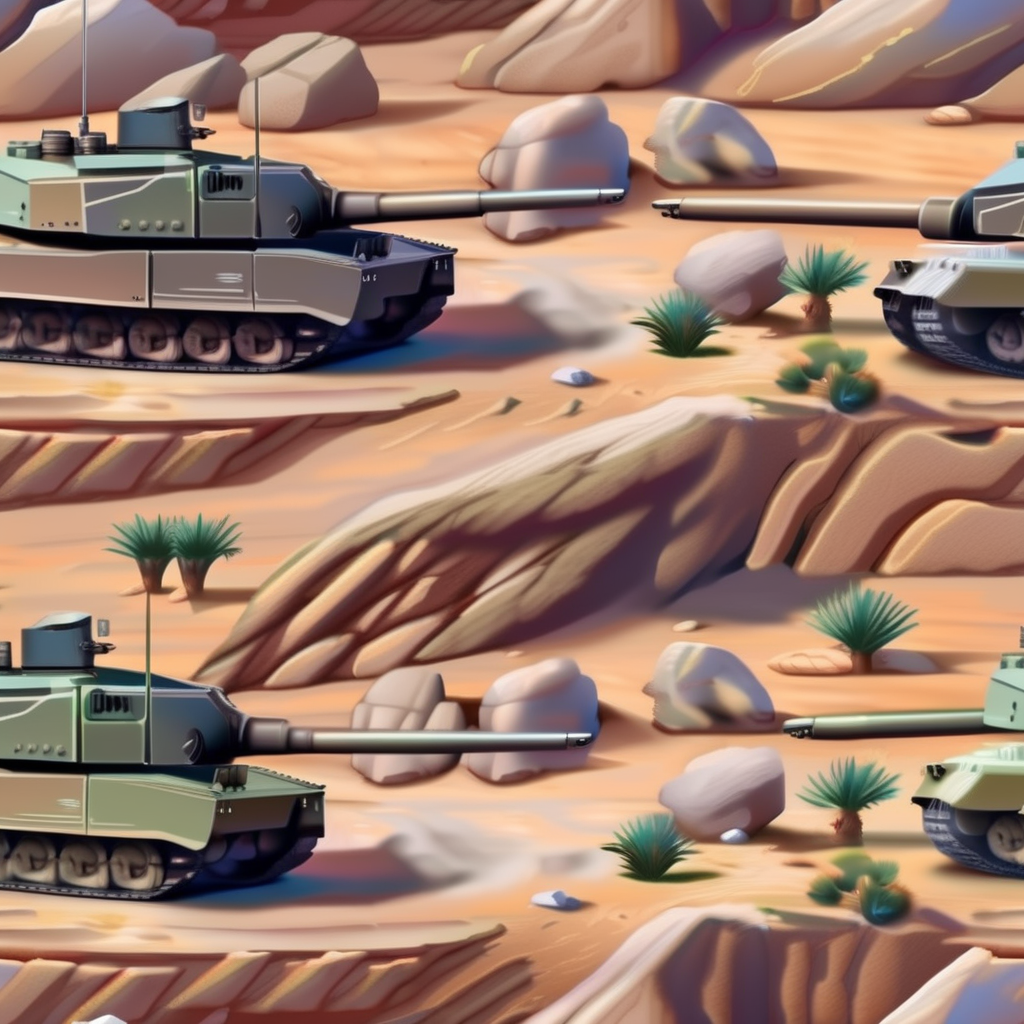
\includegraphics[width=\textwidth]{./images/xl_tank-desert-3.png}
        \caption{Dans le désert}
    \end{subfigure}
    \begin{subfigure}[b]{0.49\textwidth}
        \centering
        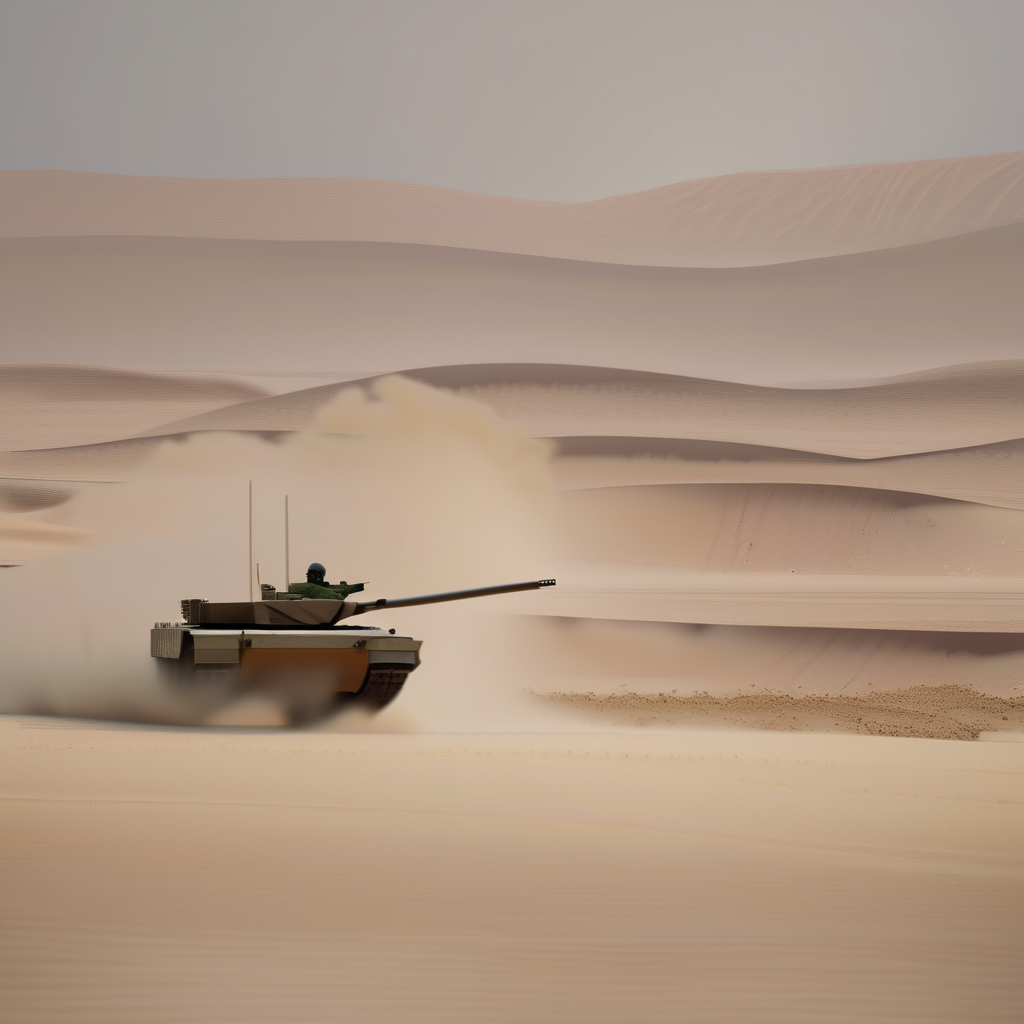
\includegraphics[width=\textwidth]{./images/xl_tank-desert_storm-2.png}
        \caption{Tempête de sable dans le désert}
    \end{subfigure}
    \hfill
    \begin{subfigure}[b]{0.49\textwidth}
        \centering
        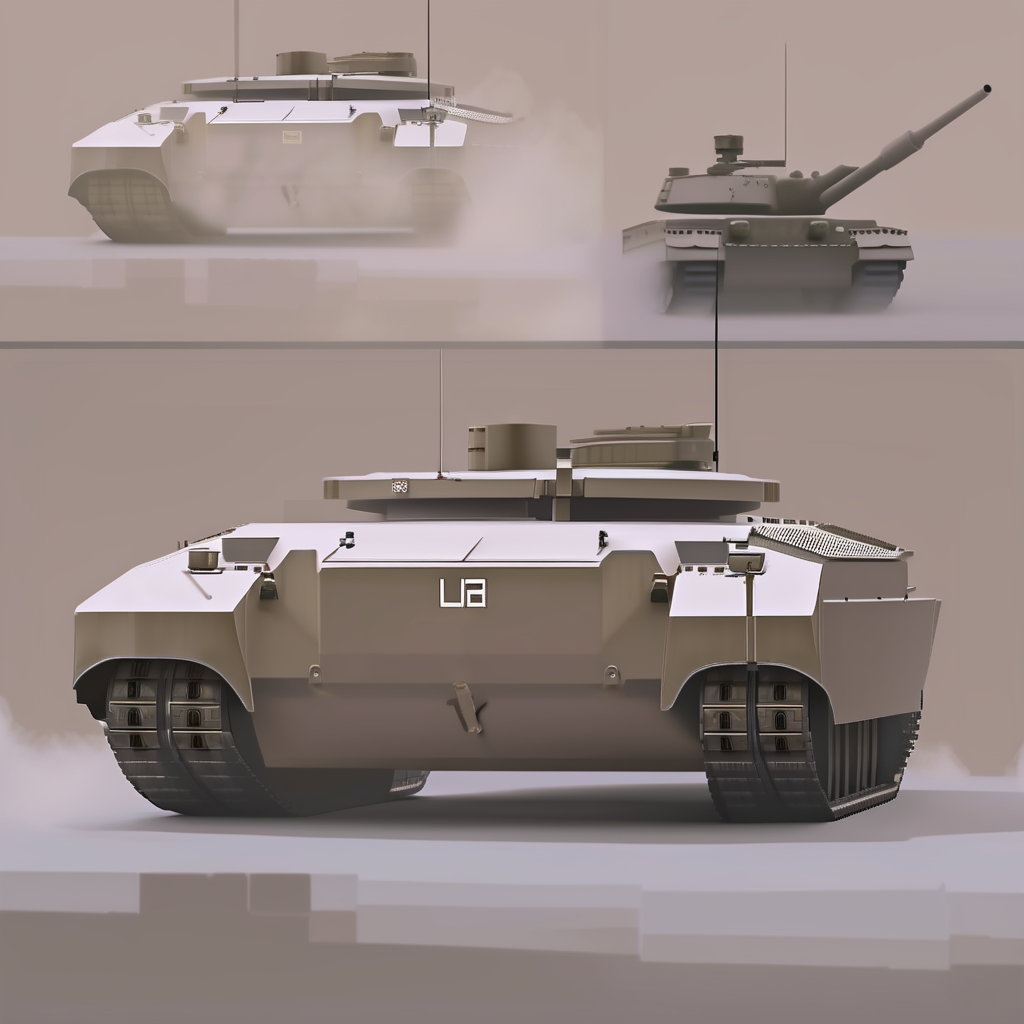
\includegraphics[width=\textwidth]{./images/xl_tank-fog-2.png}
        \caption{Dans le brouillard}
    \end{subfigure}
    \begin{subfigure}[b]{0.49\textwidth}
        \centering
        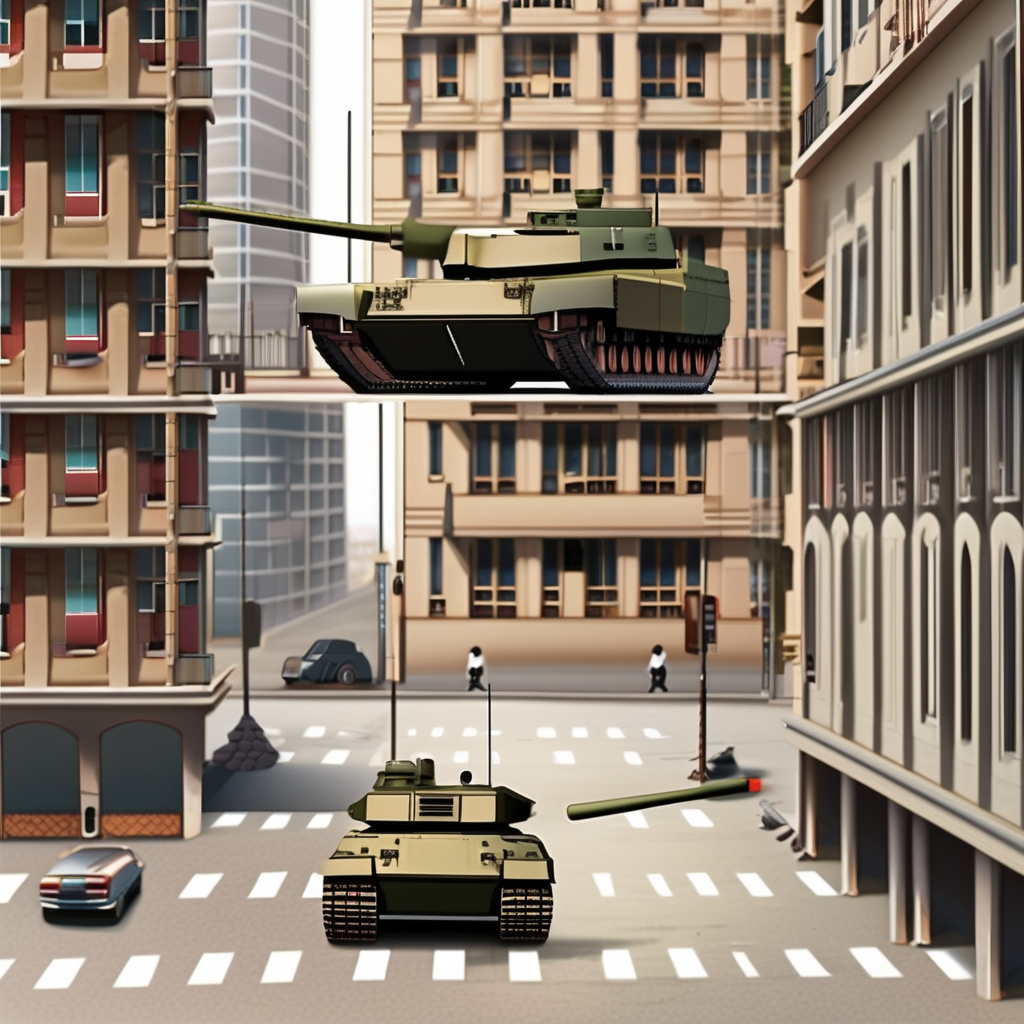
\includegraphics[width=\textwidth]{./images/xl_tank-urban_combat-1.png}
        \caption{Combat urbain}
    \end{subfigure}
    \caption{Images générés avec le modèle stable-diffusion XL}
    \label{fig:image_sdxl}
\end{figure}


Contrairement à la technique de transformation d'images, la génération d'images synthétiques ne fournit pas les anotations des véhicules présents sur les images.
Après la génération des ces images, elles doivent être validés par l'équipe de la DGA TT avant d'être annotées.

Nous continuons les expériences en modifiant les valeurs des hyperparamètres des différents modèles afin d'obtenir des images réalistes et optimales nécessaire à l'entrainement de notre modèle de detection d'objet dans les images.




\chapter*{Conclusion}
\label{chap:conclusion}
\chapter*{Conclusion}
\label{chap:conclusion}
\markboth{\MakeUppercase{Conclusion}}{}
\addcontentsline{toc}{chapter}{Conclusion}
\sloppy

Ce mémoire a permis d'explorer l'utilisation des algorithmes de deep learning pour la détection et la reconnaissance en temps réel de véhicules militaires dans des images et des vidéos.
À travers l'étude de l'état de l'art et la contribution au projet DetReco, plusieurs avancées ont été réalisées, notamment l'optimisation des modèles de détection comme YoloV8 et l'intégration de techniques de data augmentation, telles que l'utilisation de modèles génératifs comme Stable Diffusion.

L'analyse a montré que, bien que les méthodes actuelles offrent des résultats prometteurs, elles présentent encore certaines limites, notamment en termes de robustesse face à des conditions de visibilité dégradées ou de rareté des données d'entraînement.
Ces résultats soulignent l'importance de continuer à explorer des méthodes plus sophistiquées et à améliorer les jeux de données pour mieux répondre aux contraintes spécifiques du domaine militaire.

En conclusion, ce travail a posé les bases pour des recherches futures dans le domaine de la détection et de la reconnaissance en temps réel, en mettant en lumière l'importance des données de qualité et des techniques avancées de deep learning pour répondre aux exigences opérationnelles des acteurs de la défense.
Il ouvre également la voie à des collaborations renforcées entre les centres de recherche et les entités de défense pour le développement de solutions technologiques innovantes et adaptées.



\appendix
\newpage
\renewcommand{\thepage}{\Alph{page}}
\pagenumbering{Alph}


%%%%%%%%%%%%%%%%%%%%%%%%%%%%%%%%%%%%%%%%%%%%%%%%%%%%
% Don't touch this, it is auto generated
%%%%%%%%%%%%%%%%%%%%%%%%%%%%%%%%%%%%%%%%%%%%%%%%%%%%
\nocite{*}


\bibliographystyle{apalike}

\bibliography{Biblio.bib}

\cleardoublepage%

\addtocontents{toc}{\protect\setcounter{tocdepth}{4}}

\end{document}
